\documentclass{article}

\usepackage{graphicx}
\usepackage{tikz}
\usepackage{tikzsymbols}
\usetikzlibrary{calc,patterns,shapes.geometric}
\pagestyle{empty}
\usepackage[margin=0pt]{geometry}
\geometry{papersize={14in,12in}}

\def\centerarc[#1](#2)(#3:#4:#5){\draw[#1] ($(#2)+({#5*cos(#3)},{#5*sin(#3)})$) arc (#3:#4:#5);}

\begin{document}
	\begin{figure}
		\centering
		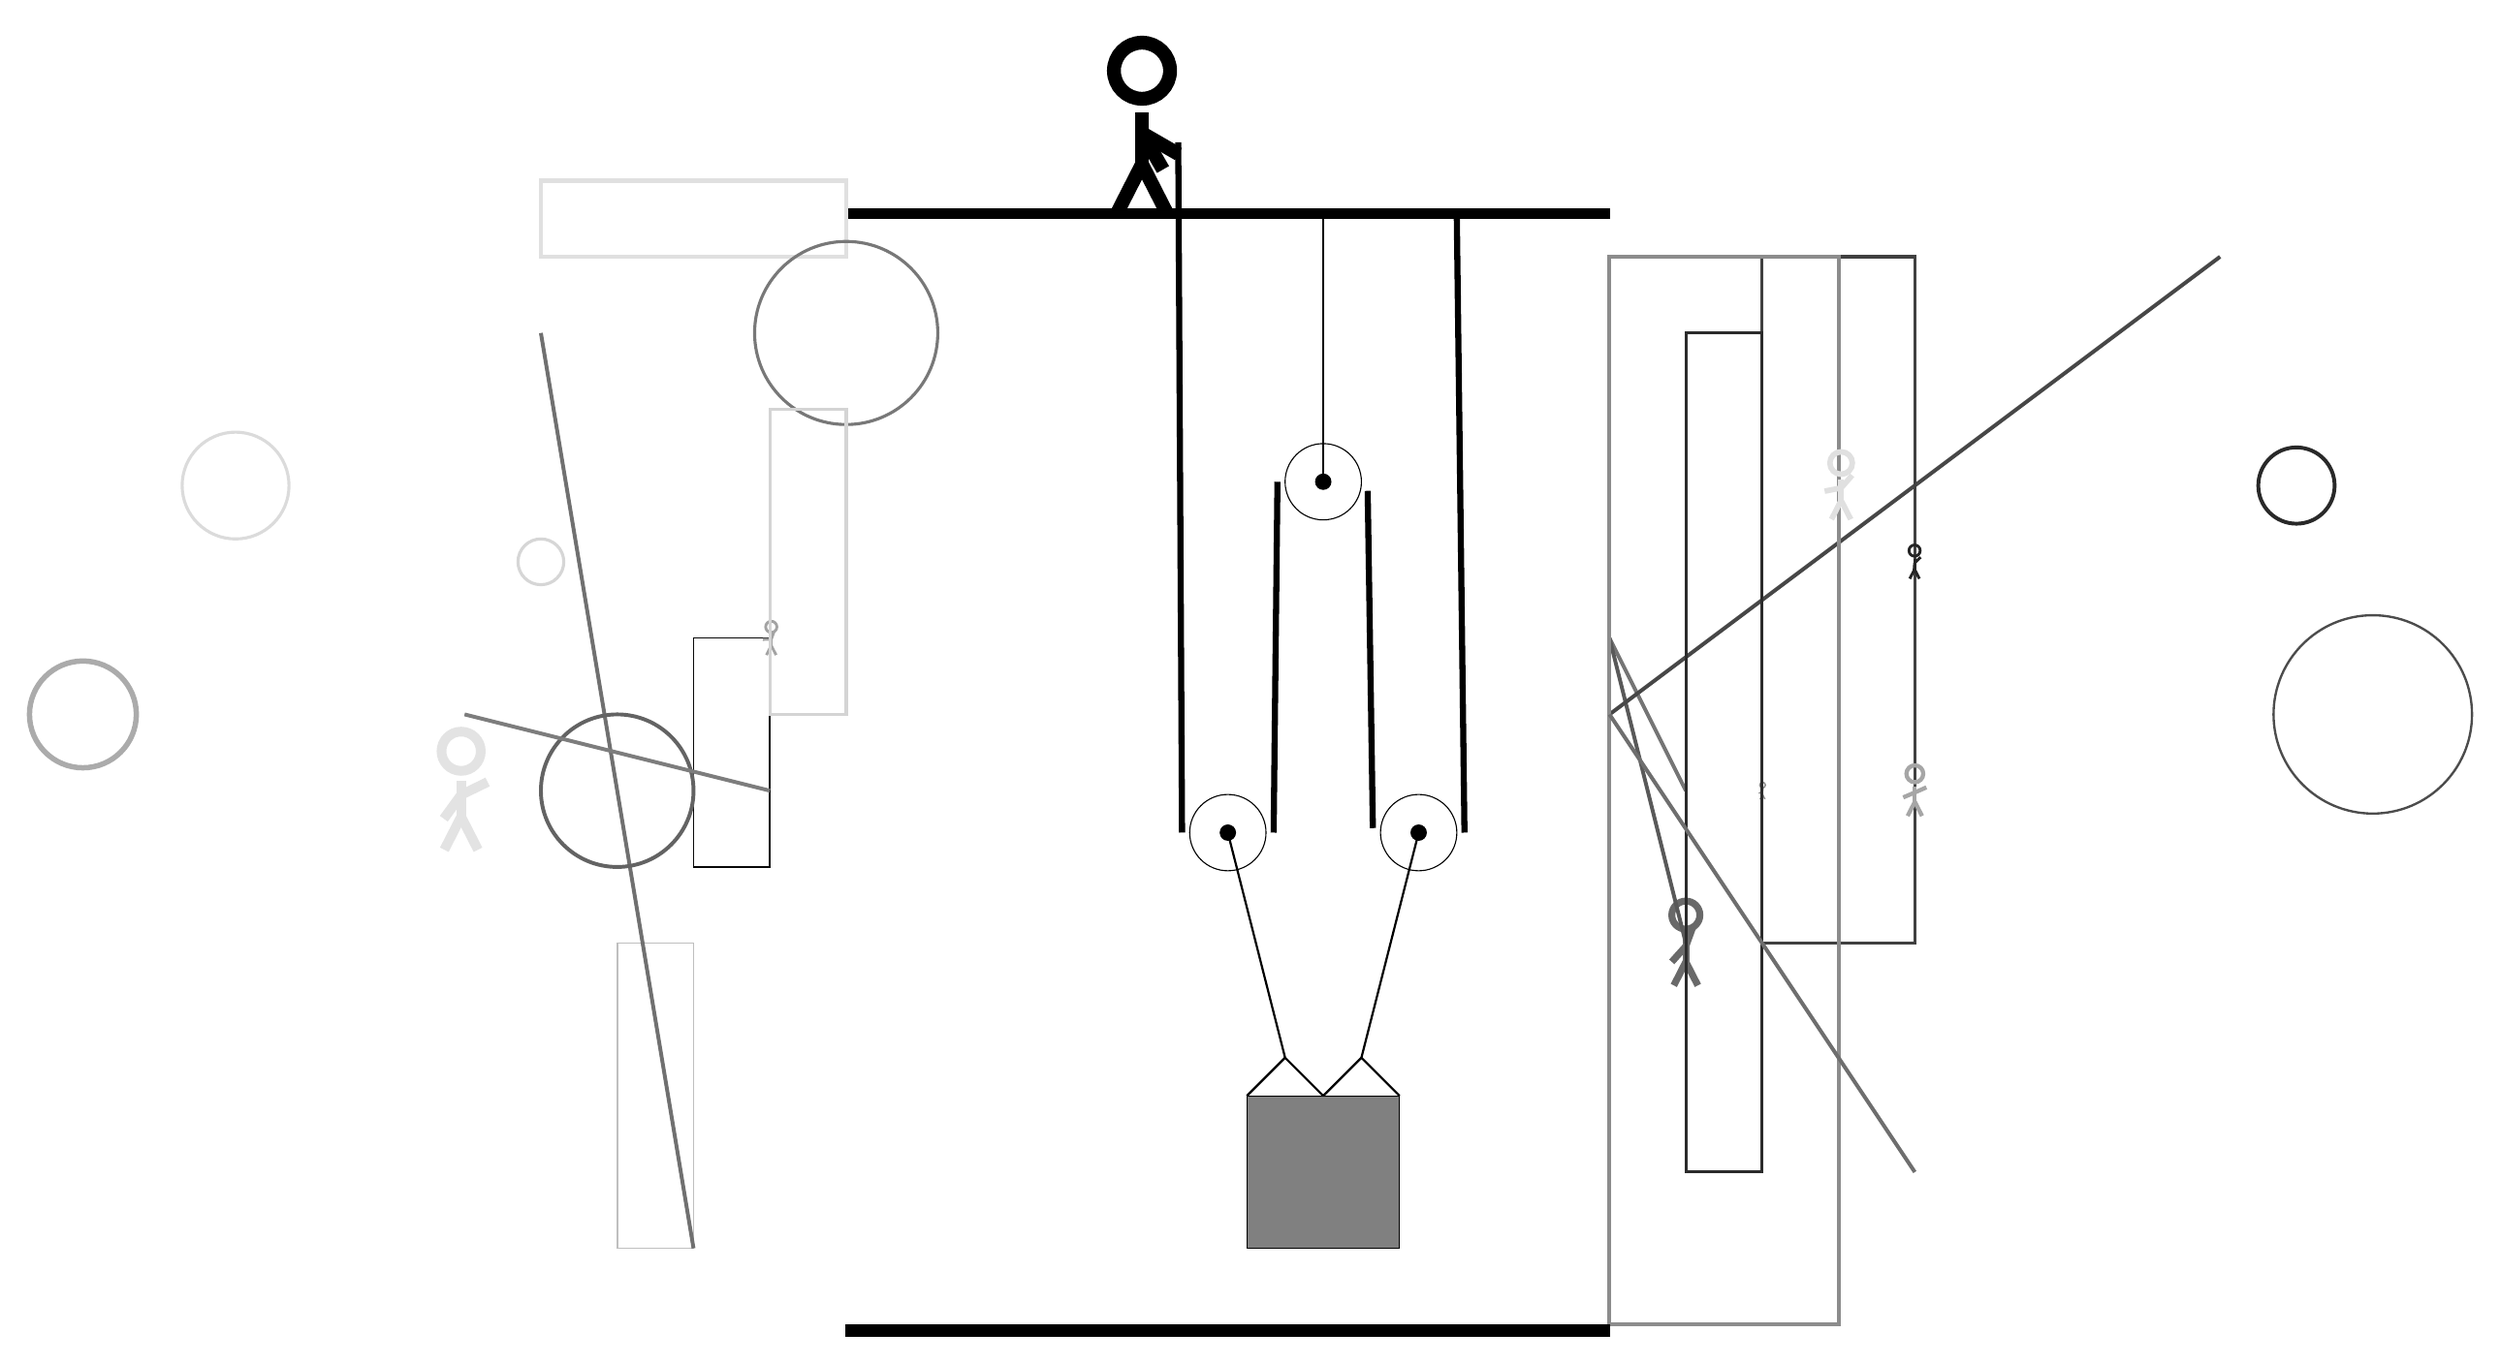
\begin{tikzpicture}
			%%%%% START %%%%%
			
			\draw[fill=black] (-4, 11.5) rectangle (6, 11.625);
			
			\draw (1, 3.45) circle (0.5);
			\draw[fill=black] (1, 3.45) circle (0.1);
			
			\draw[line width=0.5mm, color=black!54](6, 6) -- (7, 4);
			
			\draw[line width=0.2mm, color=black!97] (-5, 6) rectangle (-6, 3);
			\draw [line width=0.7mm, color=black!33](-14, 5) circle (0.7);
			\node[line width=0.3mm, color=black!59] at (7, 2) {\Strichmaxerl[5][48][70]};
			\draw[line width=0.2mm, color=black!25] (-6, -2) rectangle (-7, 2);
			\draw[line width=0.5mm, color=black!65](7, 2) -- (6, 6);
			
			\draw[line width=0.5mm, color=black!56](-8, 10) -- (-6, -2);
			
			\node[line width=0.6mm, color=black!36] at (-5, 6) {\Strichmaxerl[2][1][70]};
			\draw[line width=0.5mm, color=black!72](6, 5) -- (14, 11);
			\node[line width=0.5mm, color=black!46] at (8, 4) {\Strichmaxerl[1][30][80]};
			\draw [line width=0.5mm, color=black!61](-7, 4) circle (1.0);
			\draw [line width=0.2mm, color=black!21](8, 11) circle (0.0);
			\draw [line width=0.4mm, color=black!14](-12, 8) circle (0.7);
			\draw [line width=0.4mm, color=black!16](-8, 7) circle (0.3);
			\draw[line width=0.4mm, color=black!75] (8, 11) rectangle (10, 2);
			\draw[line width=0.5mm, color=black!45] (6, -3) rectangle (9, 11);
			
			\draw[line width=0.4mm, color=black!83] (8, 10) rectangle (7, -1);
			
			\draw[line width=0.6mm, color=black!12] (-4, 11) rectangle (-8, 12);
			\draw[line width=0.5mm, color=black!57](6, 5) -- (10, -1);
			\draw [line width=0.4mm, color=black!53](-4, 10) circle (1.2);
			\draw [line width=0.3mm, color=black!70](16, 5) circle (1.3);
			
			\node[line width=0.7mm, color=black!86] at (10, 7) {\Strichmaxerl[2][86][44]};
			
			\node[line width=0.6mm, color=black!12] at (9, 8) {\Strichmaxerl[4][11][49]};
			\node[line width=0.7mm, color=black!11] at (-9, 4) {\Strichmaxerl[7][54][26]};
			\node[line width=0.4mm, color=black!35] at (10, 4) {\Strichmaxerl[3][23][24]};
			
			\draw[line width=0.4mm, color=black!17] (-4, 5) rectangle (-5, 9);
			\draw[line width=0.5mm, color=black!51](-5, 4) -- (-9, 5);
			\draw [line width=0.5mm, color=black!84](15, 8) circle (0.5);
			
			\draw (2.25, 8.05) circle (0.5);
			\draw[fill=black] (2.25, 8.05) circle (0.1);
			\draw[thick] (2.25, 8.05) -- (2.25, 11.5);
			
			\draw (3.5, 3.45) circle (0.5);
			\draw[fill=black] (3.5, 3.45) circle (0.1);
			
			\draw[thick] (3.5, 3.45) -- (2.75, 0.5);
			\draw[thick] (1, 3.45) -- (1.75, 0.5);
			\draw[thick]  (1.25, 0) -- (1.75, 0.5) -- (2.25, 0);
			\draw[thick]  (2.25, 0) -- (2.75, 0.5) -- (3.25, 0);
			\draw[fill=black!50] (1.25, 0) rectangle (3.25, -2);
			
			\draw[line width=0.8mm] (0.35, 12.5) --  (0.4, 3.45);
			\centerarc[line width=0.8mm](1, 3.45)(180:360:0.6);
			\draw[line width=0.8mm] (1.6, 3.45) -- (1.65, 8.05);
			\centerarc[line width=0.8mm](2.25, 8.05)(-20:180:0.6);
			\draw[line width=0.8mm](2.832, 7.93) -- (2.9, 3.51);
			\centerarc[line width=0.8mm](3.5, 3.45)(160:360:0.6);
			\draw[line width=0.8mm](4.1, 3.45) -- (4.0, 11.5);
			
			\node at (-0.07, 12.7) {\Strichmaxerl[10][120][-30]};
			
			\draw[fill=black] (-4, -3) rectangle (6, -3.15);
			
			%%%%% END %%%%%
		\end{tikzpicture}
	\end{figure}	
\end{document}